\def\tutdate{24.11.2016}
\ifdefined\compileall \else
\ifdefined\compiletype
	\documentclass[handout]{beamer}
\else
	\documentclass{beamer}
	\def\compiletype{livebeamer}
\fi

\usepackage{templates/beamerthemekitwide}

\usepackage[utf8]{inputenc}
\usepackage[T1]{fontenc}
\usepackage[ngerman]{babel}
\usepackage{listings}
\usepackage{hyperref}
\usepackage{graphicx}

\usepackage{amsmath}
\usepackage{amsthm}
\usepackage{amssymb}
\usepackage{polynom}

\usepackage{ifthen}
\usepackage{adjustbox} % for \adjincludegraphics

\newcommand{\markBlue}[1]{\textcolor{kit-blue100}{#1}}
\newcommand{\markGreen}[1]{\textcolor{kit-green100}{#1}}

\newcommand{\pitem}{\pause\item}
\newcommand{\p}{\pause}

% -- MATH MACROS
\newcommand{\thistheoremname}{}
\newcommand{\G}{\mathbb{Z}}
\newcommand{\B}{\mathbb{B}}
\newcommand{\R}{\mathbb{R}}
\newcommand{\N}{\mathbb{N}}
\newcommand{\Q}{\mathbb{Q}}
\newcommand{\C}{\mathbb{C}}
\newcommand{\Z}{\mathbb{Z}}
\newcommand{\F}{\mathbb{F}}
\newcommand{\mi}{\mathrm{i}}
\renewcommand{\epsilon}{\varepsilon}


\newenvironment<>{taskblock}[1]{%
	\setbeamercolor{block title}{fg=kit-orange15,bg=kit-orange100}
	\setbeamercolor{block body}{fg=black,bg=kit-orange30}%
	\begin{block}#2{#1}}{\end{block}}

\setbeamertemplate{enumerate items}[default]

% Aussagenlogik Symbole
\newcommand{\W}{w}
\renewcommand{\F}{f}

% Kodierung
\newcommand{\frepr}{\textbf{repr}}
\newcommand{\fRepr}{\textbf{Repr}}
\newcommand{\fZkpl}{\textbf{Zkpl}}
\newcommand{\fbin}{\textbf{bin}}
\newcommand{\fdiv}{\textbf{ div }}
\newcommand{\fmod}{\textbf{ mod }}

\title[Grundbegriffe der Informatik]{Grundbegriffe der Informatik\\Tutorium 33}
\subtitle{}
\author{Lukas Bach, lukas.bach@student.kit.edu}
\date{\tutdate}

\institute{}

\titlelogo{lukasbach}

\titleimage{bg}
%\titleimage{bg-advent}


\ifthenelse{\equal{\compiletype}{livebeamer}}
	{
		\def\livebeamermode{1}
	}{}

\ifthenelse{\equal{\compiletype}{print}}
	{
		\def\printmode{1}
	}{}

\setbeamercovered{invisible}

%\usepackage[citestyle=authoryear,bibstyle=numeric,hyperref,backend=biber]{biblatex}
%\addbibresource{templates/example.bib}
%\bibhang1em

\begin{document}
	
\selectlanguage{ngerman}


%title page
\begin{frame}
	\titlepage
\end{frame}

%table of contents
\ifdefined\printmode
	\ifdefined\compileall \else
	\begin{frame}{Gliederung}
		\tableofcontents
	\end{frame}
\fi\fi

\fi

\section{Übersetzungen}

\begin{frame} {Übersetzungen}
	\begin{block} {Definition der Semantikabbildung}
		Sei \textit{Sem} die Menge der Bedeutungen. \p Ferner seien $A$ und $B$ Alphabete \p und $L_A \subseteq A^* \text{ und } L_B \subseteq B^*$.\\
		\p Weiter sei $sem_A:L_A \rightarrow Sem$ \p und $sem_B: L_B \rightarrow Sem$\\
		\p Dann heißt $f: L_A \rightarrow L_B$ Übersetzung \p , wenn gilt: für jedes $w \in L_A$ gilt $sem_A(w) = sem_B(f(w))$.
	\end{block}
	\begin{itemize}
		\pitem Bedeutungserhaltende Abbildungen von Wörtern auf Wörter
	\end{itemize}
	\textbf{Beispiel}\\
	\p Betrachte $Trans_{2,16}: \mathbb{Z}_{16}^* \rightarrow \mathbb{Z}_{2}^*$ mit $ Trans_{2,16}(w) = Repr_2(Num_{16}(w))$
	\begin{itemize}
		\pitem $Trans_{2,16}(A3) = Repr_2(Num_{16}(A3)) = Repr_2(163) = 10100011$
	\end{itemize}
\end{frame}
\begin{frame}{Wozu Übersetzungen}
	\begin{itemize}
		\pitem Lesbarkeit (vergleiche $DF_{16}$ mit $11011111_2$)
		\pitem Verschlüsselung
		\pitem Kompression (Informationen platzsparend aufschreiben)
		\pitem Kontextabhängige Semantiken (Deutsch $\rightarrow$ Englisch)
		\pitem Fehlererkennung
	\end{itemize} 
\end{frame}


\begin{frame}{Codierungen}	
	\begin{block}{Definitionen}
		\begin{itemize}
			\pitem Codewort $f(w)$ \p einer Codierung $f: L_A \rightarrow L_B$
			\pitem Code: $\{f(w)|w \in L_A\} = f(L_A)$
			\pitem Codierung: \textbf{Injektive} Übersetzung
			\begin{itemize}
				\pitem Ich komme immer eindeutig von einem Codewort f(w) zu $w$ zurück
			\end{itemize}
		\end{itemize}
	\end{block}\p
	\textbf{Bemerkung}\\
	\begin{itemize}
		\pitem Was ist, wenn $L_A$ unendlich ist (man kann nicht alle Möglichkeiten aufzählen)
		\pitem Auswege: Homomorphismen, Block-Codierungen
	\end{itemize}
\end{frame}


\subsection{Homomorphismen}

\begin{frame}{Homomorphismen}
	\begin{block} {Definition von Homomorphismen}\p
		Seien $A, B$ Alphabete. \p Dann ist $h: A^* \rightarrow B^*$ \p ein Homomorphismus\p , falls für alle $w_1, w_2 \in A^*$ gilt:\\ \p
		\begin{equation*}
		h(w_1w_2) = h(w_1)h(w_2)
		\end{equation*}
	\end{block}

	\begin{itemize}
		\pitem Ein Homomorphismus ist Abbildung, die mit Konkatenation verträglich ist
		\pitem Homomorphismus ist $\varepsilon$-frei, wenn für jedes $x \in A: h(x) \neq \varepsilon$
		\pitem Homomorphismen lassen das leere Wort unverändert, also $h(\varepsilon) = \varepsilon$
	\end{itemize}
\end{frame}

\begin{frame}
	Sei $h$ ein Homomorphismus.
	
	\begin{taskblock}{Übung zu Homomorphismen}
			\begin{enumerate}
				\pitem $h(a) = 001$ und $h(b) = 1101$. Was ist dann $h(bba)$? 
				\pitem[$\rightarrow$] $h(bba) = h(b)h(b)h(a) = 1101 \cdot 1101 \cdot 001 = 11011101001$
				\pitem Sei $h(a) = 01, h(b) = 11 \text{ und } h(c) = \varepsilon$. Nun sei $h(w)= 011101$. Was war $w$? 
				\pitem[$\rightarrow$] $aba$ oder $cabccac$, ... Allgemein: $w \in \{c\}^* \cdot \{a\} \cdot \{c\}^* \cdot \{b\} \cdot \{c\}^* \cdot \{a\} \cdot \{c\}^*$ \\ \p $\epsilon$-Freiheit hat also die Eindeutigkeit zerstört!
				\pitem Kann h aus 2 eine Codierung sein?
				\pitem[$\rightarrow$] Nein, da nicht injektiv!
				\pitem Warum will man $\varepsilon$-freie Homomorphismen?
				\pitem[$\rightarrow$] Information geht sonst verloren!
				\pitem Was heißt hier "Information geht verloren"? 
				\pitem[$\rightarrow$] Es gibt $w_1 \neq w_2$ mit $h(w_1) = h(w_2)$
			\end{enumerate}
	\end{taskblock}
\end{frame}

\begin{frame}
	\begin{itemize}
		\pitem Information kann auch anders "verloren" gehen
		\pitem[$\rightarrow$] z.B. $h(a) = 0, h(b) = 1, h(c) = 10$ \p -- Wie das?
	\end{itemize} \pause
	\begin{block}{Präfixfreiheit}
		\p Gegeben ist ein Homomorphismus $h: A^* \rightarrow B^*$.\\
		\p Wenn für keine zwei verschiedenen $x_1, x_2 \in A$ gilt\p , dass $h(x_1)$  Präfix von $h(x_2)$ ist\p , dann ist $h$ präfixfrei. 
	\end{block}
	\pause
	\begin{block}{Satz}
		Präfixfreie Codes sind injektiv.
	\end{block} \pause
	\textbf{Beispiele}\\
	\begin{itemize}
		\pitem $h(a) = 01 \text{ und } h(b) = 1101 $ ist präfixfrei
		\pitem $g(a) = 01 \text{ und } g(b) = 011$ ist nicht präfixfrei
	\end{itemize}
\end{frame}

\subsection{Huffman Codierung}

\begin{frame}{Huffman-Codierung}
	\begin{itemize}
		\pitem Komprimiert eine Zeichenkette
		\pitem Kodiert häufiger vorkommende Zeichen zu kürzeren Codewörter als Zeichen die seltener vorkommen.
		\pitem Vorgehensweise:
		\begin{enumerate}
			\pitem Zähle Häufigkeiten aller Zeichen der Zeichenkette
			\pitem Schreibe alle vorkommenden Zeichen und ihre Häufigkeiten nebeneinander
			\pitem Wiederhole, bis der Baum fertig ist:
			\begin{itemize}
				\pitem Verbinde die zwei Zeichen mit niedrigsten Häufigkeiten zu neuem Knoten über diesen
				\pitem Dieser hat als Zahl die aufsummierte Häufigkeiten
			\end{itemize}
			\pitem Danach: Alle linken Kanten werden mit $0$ kodiert, alle rechten Kanten mit $1$
		\end{enumerate}
	\end{itemize}

	\p Das Ergebnis ist eine Zeichenkette aus $\{0,1\}$\p , die kürzer ist als die ursprüngliche Zeichenkette in binär.
\end{frame}

\begin{frame}{Huffman-Codierung}
	Gegeben
	\begin{itemize}
		\item $w \in A^*$ 
		\only<1>{ \\ }\textbf{w } = \texttt{ afebfecaffdeddccefbeff }
		\pause
		\item Anzahl der Vorkommen aller Zeichen in w ($N_x(w)$)
	\end{itemize}		
	\only<2>{
		\textbf{Häufigkeiten:}\\
		\begin{tabular}{c c c c c c c}
			\hline
			x &a&b&c&d&e&f\\
			\hline
			$N_x(w)$& 2& 2&3&3& 5& 7\\
			\hline
		\end{tabular}							
	}
	\pause
	Zwei Phasen zur Bestimmung eines Huffman-Codes
	\begin{enumerate}
		\item Konstruieren eines "Baumes"
		\begin{itemize}
			\item Blätter entsprechen den Zeichen
			\item Kanten mit 0 und 1 beschriften\\ 
			\only<3>{
				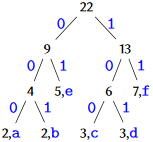
\includegraphics[scale=0.8]{images/Baum.PNG}
				\begin{tabular}{c c c c c c c}
					\textbf{Häufigkeiten:}\\
					\hline
					x  &a&b&c&d&e&f\\
					\hline
					$N_x(w)$& 2& 2&3&3& 5& 7\\
					\hline
				\end{tabular}	
			}
		\end{itemize} 
		\pause
		\item Ablesen der Codes aus dem Baum (Pfadbeschriftungen)
	\end{enumerate}
	\only<4>{
		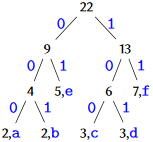
\includegraphics[scale=0.46]{images/Baum.png}
		\hspace{0.4cm}
		\begin{tabular}{c c c c c c c}
			\textbf{Häufigkeiten:}\\
			\hline
			x &a&b&c&d&e&f\\
			\hline
			$N_x(w)$ & 2& 2&3&3& 5& 7\\
			
			\textbf{Codewörter:}\\
			\hline
			x &a&b&c&d&e&f\\
			\hline
			h(x)& 000& 001&100&101& 01& 11\\
			\hline
		\end{tabular}							
	}		
\end{frame}

\begin{frame}{Übung zu Huffman Codierung}
	\begin{taskblock}{Übung}
		Sei $A = \{$\texttt a, b, c, d, e, f, g, h$\}$\\
		\begin{itemize}
			\item Codiere das Wort \texttt{badcfehg} mit Hilfe der Huffman-Codierung \pause
			\item [$\rightarrow$]Mögliche Lösung: 001 100 010 011 101 000 111 110
			\pause
			\item Wie lauten die Codewörter, wenn für das Wort $w$ gilt: $N_a(w) = 1, N_b(w) = 2, N_c(w) = 2, N_d(w) =8, N_e(w) =16, N_f(w) =32, N_g(w) = 64, N_h(w) = 128$
			
		\end{itemize} \pause
		Mögliche Lösung:\\
		\begin{tabular}{|c|c c c c c c c c|}
			\hline
			x &a&b&c&d&e&f&g&h\\
			\hline
			h(x)& 0000000& 0000001&000001&00001& 0001&001& 01&1\\
			\hline
		\end{tabular}
	\end{taskblock}
\end{frame}	

	\begin{frame}
	\begin{itemize}
		\item Wie lang wäre das zweite Wort (\texttt{abbcccc} $\texttt{d}^{8}$...$\texttt{g}^{64}\texttt{h}^{128}$) mit dem ersten Code codiert? 
		\pause
		\item[$\rightarrow$] 741 Symbole. Also dreimal so lang wie das Original. \pause
		\item Wie lang wäre das zweite Wort mit dem zweiten Code codiert?\pause
		\item[$\rightarrow$] 501 Symbole. Also nur zweimal so lang wie das Original. \pause
		\item Was fällt euch auf?
	\end{itemize}
\end{frame}		

\begin{frame}{Wahr oder falsch?}
	Sei $h: A^* \rightarrow \mathbb{Z}_2$ eine Huffman-Codierung
	\begin{itemize}
		\item h ist ein $\varepsilon$-freier Homomorphismus \pause \textbf{Wahr!}\pause
		\item Häufigere Symbole werden mit langen Worten codiert, seltene mit kürzeren \pause \textbf{Falsch!}\pause
		\item Die Kompression ist am stärksten, wenn die Häufigkeiten aller Zeichen ungefähr gleich sind. \pause \textbf{Falsch!} \pause
		\item h ist präfixfrei \pause \textbf{Wahr!} \pause
		\item Es kann noch kürzere Codierungen geben \pause \textbf{Falsch!}
	\end{itemize}
\end{frame}

	
\begin{frame}{Huffman-Codierung}
	\begin{block}{Eigenschaften}
		Sei $A$ ein Alphabet und $w \in A$. Dann gilt für die Huffman-Codierung h:
		\begin{itemize}
			\item $h: A^* \rightarrow \mathbb{Z}_2$
			\item $h$ ist $\varepsilon$-freier Homomorphismus
			\item $h$ ist präfixfreier Homomorphismus
			\item Häufigere Symbole werden mit kurzen Worten codiert, seltene mit längeren
			\item Produziert kürzestmögliche Codierungen
		\end{itemize}
	\end{block}
\end{frame}

\begin{frame}{Block-Codierung mit Huffman}
	\begin{itemize}
		\pitem Wir betrachten nicht mehr einzelne Symbole, sondern Blöcke von fester Länge $b > 1$
		\pitem Blätter des Huffman-Baums sind jetzt \textit{Wörter der Länge b}
	\end{itemize}

	\vspace{.5cm}
	
	Beispiel an der Tafel: Codierung von $aab\cdot deg \cdot deg \cdot aab \cdot ole \cdot aab \cdot deg \cdot aab$.\p
	
	\vspace{.5cm}
	
	\p
	\begin{itemize}
		\pitem Alphabet $A =\{$\texttt{a,b,c,d} $\}$
		\pitem Text über $A$, der nur aus Teilwörtern der Länge 10 zusammengesetzt ist, in denen jeweils immer nur ein Symbol vorkommt
		%\item z.B. \texttt{aaaaaaaaaabbbbbbbbbbcccccccccc}...
		\pitem Angenommen $\texttt{a}^{10}$, ..., $\texttt{d}^{10}$ kommen alle gleich häufig vor. Wie lang ist dann die Huffman-Codierung? \pause
		\pitem[$\rightarrow$] Ein Fünftel, weil jeder Zehnerblock durch zwei Bits codiert wird
	\end{itemize}
	
\end{frame}



\section{Speicher}


\begin{frame}{Speicher}
	\begin{itemize}
		\pitem Ein \textbf{Bit} ist Zeichen aus $A = \{0, 1\}$
		\pitem Ein \textbf{Byte} ist ein Wort aus acht Bits
		\pitem Abkürzungen
		\begin{itemize}
			\pitem Für Bit: \texttt{bit}
			\pitem Für Byte: \texttt{B}
		\end{itemize}
	\end{itemize}
\end{frame}

\begin{frame}{Präfixe}
	\begin{center}
		\textbf{Dezimal}\\
		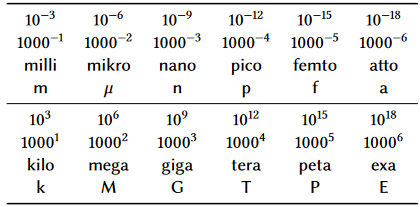
\includegraphics[scale=0.6]{images/dezimal.png}\\ \pause
		\textbf{Binär}\\
		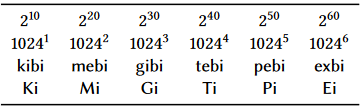
\includegraphics[scale=0.6]{images/binaer.png}
	\end{center}
	
\end{frame}

\begin{frame}{Gesamtzustand eines Speichers}
	\p Zu jedem Zeitpunkt ist
	\begin{itemize}
		\pitem für jede \markBlue{Adresse} festgelegt, welcher \markBlue{Wert} dort ist
		\pitem beides meist Bitfolgen
	\end{itemize}
	\p Vorstellung: Tabelle mit zwei Spalten\\
	\begin{center}
		\begin{tabular}{|l l|}
			\hline
			\textbf{Adresse} & \textbf{Wert} \\
			\hline
			Adresse 1& Wert 1 \\
			Adresse 2 & Wert 2 \\
			Adresse 3 & Wert 3 \\
			...&...\\
			Adresse n & Wert n\\
			\hline
		\end{tabular}
	\end{center}
\end{frame}

\begin{frame}{Zustand eines Speichers -- formal}
	\p\begin{block}{Definition des Speicherzustandes}
		Sei $Adr$ die Menge aller Adressen und $Val$ die Menge aller Werte.\\
		Dann ist \\ \begin{center}
			$m: Adr \rightarrow Val$
		\end{center}
		der aktuelle Zustand des Speichers. Dabei ist $m(a)$ der aktuelle Wert an der Adresse $a$.
	\end{block}
\end{frame}


\begin{frame}{Lesen und Speichern}
	\pause
	\begin{block}{$Mem$}
		Menge aller möglichen Speicherzustände, also Menge aller Abbildungen von $Adr$ nach $Val$
		\begin{center}
			$Mem:= Val^{Adr}$
		\end{center}
	\end{block}
	\p Anmerkung: \p Für zwei Mengen $A$, $B$ gilt\p : $A^B := \{f: B \rightarrow A\}$.\p
	\begin{block}{$memread$}
		\begin{center}
			$memread: Mem \times Adr \rightarrow Val \text{ mit } (m, a) \mapsto m(a)$
		\end{center}
	\end{block}
	\pause
	\begin{block}{$memwrite$}
		$memwrite: Mem \times Adr \times Val \rightarrow Mem \text{ mit } (m, a,v) \mapsto m'$\\
		Für $m'$ wird folgendes gefordert:
		\begin{center}
			$m(a') :=\begin{cases} 
			v& \text{ falls } a' = a\\
			m(a') &\text{ falls } a' \neq a
			\end{cases} $ 
		\end{center}
	\end{block}
\end{frame}

\begin{frame}{Eigenschaften von $memread$ und $memwrite$}
	
	\begin{block}{Eigenschaften (``Invarianten'')}
		\begin{itemize}
			\pitem $memread(memwrite(m,a,v),a) = v$ \p (Also: An $a$ einen Wert $v$ zu schreiben und danach bei $a$ zu lesen gibt den Wert $v$ zurück \p $\Rightarrow$ Konsistente Datenhaltung)
			\pitem $memread(memwrite(m, a', v'),a) = memread(m,a)$ \p (Also: Auslesen einer Speicherstelle ist unabhängig davon, was vorher an eine andere Adresse geschrieben wurde \p $\Rightarrow$ Unabhängige Datenhaltung)
		\end{itemize}
	\end{block}

\end{frame}

\begin{frame}
	\textbf{Aufgaben}\\
	Aktueller Speicherzustand: \\
	\vspace{0.2cm}
	\begin{tabular}{|c| c|}
		\hline
		Adresse & Wert\\
		\hline
		00000& 01110\\
		00001& 00100\\
		00010& 00111\\
		00011& 00000\\
		...& ...\\
		\hline
	\end{tabular}\\
	\vspace{0.3cm}
	Was ist?
	\begin{itemize}
		\item $memread(memwrite(m, memread(m, 00011), 01010), 00000)$ \pause
		\item[$\rightarrow$] 01010
	\end{itemize}
	
\end{frame}

\ifdefined\compileall
\else


\ifthenelse{\equal{\compiletype}{print}}
{

\begin{frame}{Informationen}
	
	\begin{columns}
		\begin{column}{0.5\textwidth}
			
			\begin{block}{Zum Tutorium}
				\begin{itemize}
					\item Lukas Bach
					\item Tutorienfolien auf: 
					\begin{itemize}
						\item \url{http://gbi.lukasbach.com}
					\end{itemize}
					\item Tutorium findet statt:
					\begin{itemize}
						\item Donnerstags, 14:00 - 15:30
						\item 50.34 Informatikbau, -107
					\end{itemize}
				\end{itemize}
			\end{block}
			
			\begin{block}{Mehr Material}
				\begin{itemize}
					\item Ehemalige GBI Webseite:
					\begin{itemize}
						\item \url{http://gbi.ira.uka.de}
						\item Altklausuren!
					\end{itemize}
				\end{itemize}
			\end{block}
			
		\end{column}
		\begin{column}{0.5\textwidth}
			
			\begin{block}{Zur Veranstaltung}
				\begin{itemize}
					\item Grundbegriffe der Informatik
					\item Klausurtermin:
					\begin{itemize}
						\item 06.03.2017, 11:00
						\item Zwei Stunden Bearbeitungszeit
						\item 6 ECTS für Informatiker und Informationswirte, 4 ECTS für Mathematiker und Physiker
					\end{itemize}
				\end{itemize}
			\end{block}
			
			\begin{block}{Zum Übungsschein}
				\begin{itemize}
					\item Übungsblatt jede Woche
					\item Ab 50\% insgesamt hat man den Übungsschein
					\item Keine Voraussetzung für die Klausur, aber für das Modul
				\end{itemize}
			\end{block}
			
		\end{column}
	\end{columns}
	
\end{frame}

}{}

\ifdefined\livebeamermode
	\begin{frame}
		
\includegraphics[width=\linewidth]{images/thatsall.png}
	\end{frame}
\fi

\end{document}

\fi